\documentclass[a4paper]{article}

\usepackage{fullpage} % Package to use full page
\usepackage{parskip} % Package to tweak paragraph skipping
\usepackage{tikz} % Package for drawing
\usepackage{amsmath}
\usepackage{hyperref}

\usepackage{listings}
\usepackage{xcolor}

\definecolor{mygreen}{rgb}{0,0.6,0}
\definecolor{mygray}{rgb}{0.5,0.5,0.5}
\definecolor{mymauve}{rgb}{0.58,0,0.82}
\lstset{ %
  backgroundcolor=\color{white},   % choose the background color
  basicstyle=\footnotesize,        % size of fonts used for the code
  breaklines=true,                 % automatic line breaking only at whitespace
  captionpos=b,                    % sets the caption-position to bottom
  commentstyle=\color{mygreen},    % comment style
  escapeinside={\%*}{*)},          % if you want to add LaTeX within your code
  keywordstyle=\color{blue},       % keyword style
  stringstyle=\color{mymauve},     % string literal style
}

\title{CSCE 569: Homework 1}
\author{Nick Tyler}
\date{02/09/18}

\begin{document}

\maketitle

\section*{Matrices and Vectors}
Matrices and vectors are very common in scientific applications, especially in physics where solving systems of equations in N dimensions is aided by the use of matrices. Matrices, vectors, and their products are seen in many physics equations, from solving for moments of inertia of spinning objects in classical mechanics, to the Hamiltonian of a harmonic oscillators in quantum mechanics. Because of this, many scientific applications which use computers often use matrix and vector multiplication to numerically solve systems of physics equations.

\section{Matrix Matrix Multiplication}
Mathematically matrix multiplication between two matrices, A and B size M$\times$L and L$\times$N respectfully, to form the resultant matrix C with size M$\times$N, is shown below.
\[
\begin{bmatrix}
    c_{11}  &  c_{12} & c_{13}  & \cdots \\
    c_{21}  &  c_{22} & c_{23}  & \cdots \\
    c_{31}  &  c_{32} & c_{33}  & \cdots \\
    \vdots & \vdots & \vdots & \ddots 
\end{bmatrix} 
=
\begin{bmatrix}
    a_{11}  &  a_{12} & a_{13} & \cdots  \\
    a_{21}  &  a_{22} & a_{23} & \cdots  \\
    a_{31}  &  a_{32} & a_{33} & \cdots  \\
    \vdots & \vdots & \vdots & \ddots 
\end{bmatrix}
\begin{bmatrix}
    b_{11}  &  b_{12} & b_{13} & \cdots  \\
    b_{21}  &  b_{22} & b_{23} & \cdots  \\
    b_{31}  &  b_{32} & b_{33} & \cdots  \\
    \vdots & \vdots & \vdots & \ddots 
\end{bmatrix}
\]

With the elements of the resulting matrix C defined by:

\begin{equation*}
c_{ij} = \sum_{k} a_{ik}b_{kj}
\end{equation*}

The mathematical, row major representation can be translated into an algorithm as seen below, where the new element of C is calculated by taking the values of the i'th row of matrix A and j'th column of matrix B multiplying them together and then adding them to a temporary value. The row of A and column of B are then walked through, multiplied together and then summed until all columns of A and rows of B are accounted for.

\begin{lstlisting}[language=C++]
for (i = 0; i < N; i++){
  for (j = 0; j < M; j++) {
    float temp = 0.0;
    for (w = 0; w < K; w++)
      temp += A[i * K + w] * B[w * M + j];
    C[i * M + j] = temp;
  }
}
\end{lstlisting}


Depending on how the matrix is stored in memory the algorithm must be modified slightly. The skeleton of the algorithm stays the same, the only change is to how the elements of A and B are accessed in memory. This modification to the fifth line of the algorithm can be seen below.

\begin{lstlisting}[language=C++]
// A Row, B Row
temp += A[i * K + w] * B[w * M + j];
// A Col, B Row      
temp += A[w * K + i] * B[w * M + j];
// A Row, B Col         
temp += A[w * K + i] * B[j * M + w];
// A Col, B Col       
temp += A[i * K + w] * B[j * M + w];
\end{lstlisting}

\section{Matrix Vector Multiplication}
Matrix vector multiplication is just a special case of matrix multiplication where a matrix A of size M$\times$N is multiplied with a matrix B of size N$\times$1, resulting in a matrix C of size M$\times$1.

\[
\begin{bmatrix}
    c_{1} \\
    c_{2} \\
    c_{3} \\
    \vdots  
\end{bmatrix} 
=
\begin{bmatrix}
    a_{11}  &  a_{12} & a_{13} & \cdots  \\
    a_{21}  &  a_{22} & a_{23} & \cdots  \\
    a_{31}  &  a_{32} & a_{33} & \cdots  \\
    \vdots & \vdots & \vdots & \ddots 
\end{bmatrix}
\begin{bmatrix}
    b_{1}  \\
    b_{2}  \\
    b_{3}  \\
    \vdots
\end{bmatrix}
\]
Again the elements of C are defined similarly with a summation over the products of the two matrices as shown below:
\begin{equation*}
c_{i} = \sum_{k} a_{ik}b_{k}
\end{equation*}

And with an algorithm, as:

\begin{lstlisting}[language=C++]
for (i = 0; i < M; i++) {
  float temp = 0.0;
  for (j = 0; j < N; j++) {
    temp += A[i * N + j] * B[j];
  }
  C[i] = temp;
}
\end{lstlisting}

And once again the elements of A can be stored in row major or column major with the differences between how the elements of the matrix are stored and accessed in memory, changing how to access the elements of A is all that is needed.

\begin{lstlisting}[language=C++]
// A Row major
temp += A[i * N + j] * B[j];
// A Col Major
temp += A[j * N + i] * B[j];
\end{lstlisting}

\pagebreak
\section*{Performance}
All performance results are from my personal computer running Ubuntu 17.10, Artful, with 16GB of ram and the following cpu configuration.

\begin{verbatim}
Architecture:        x86_64
CPU op-mode(s):      32-bit, 64-bit
Byte Order:          Little Endian
CPU(s):              8
On-line CPU(s) list: 0-7
Thread(s) per core:  2
Core(s) per socket:  4
Socket(s):           1
NUMA node(s):        1
Vendor ID:           GenuineIntel
CPU family:          6
Model:               58
Model name:          Intel(R) Core(TM) i7-3770 CPU @ 3.40GHz
Stepping:            9
CPU MHz:             3400.264
CPU max MHz:         3900.0000
CPU min MHz:         1600.0000
BogoMIPS:            6800.52
Virtualization:      VT-x
L1d cache:           32K
L1i cache:           32K
L2 cache:            256K
L3 cache:            8192K
NUMA node0 CPU(s):   0-7
\end{verbatim}

The programs for Matrix Matrix and Matrix Vector multiplication were tested both with and without gcc optimization's. With gcc optimization's enabled (-O3) the compiler will attempt to optimize the executable for speed. There are many flags which are enabled with optimization but most likely one of the optimization's involving loop unraveling or vectorization are what helps to speed up the results. All the information on what the optimization and all the flags enabled was found at the \href{https://gcc.gnu.org/onlinedocs/gcc/Optimize-Options.html}{online gcc optimization manual}.

The performance for matrix multiplication can be seen in the following graph. The worst performance came from A column major and B row major at 2048 with no optimization, and even with optimization's enabled it was not fast in it's execution time. However storing the matrices as column major gives the best performance, it is the fastest method both with and without optimization's enabled.
\begin{center}
    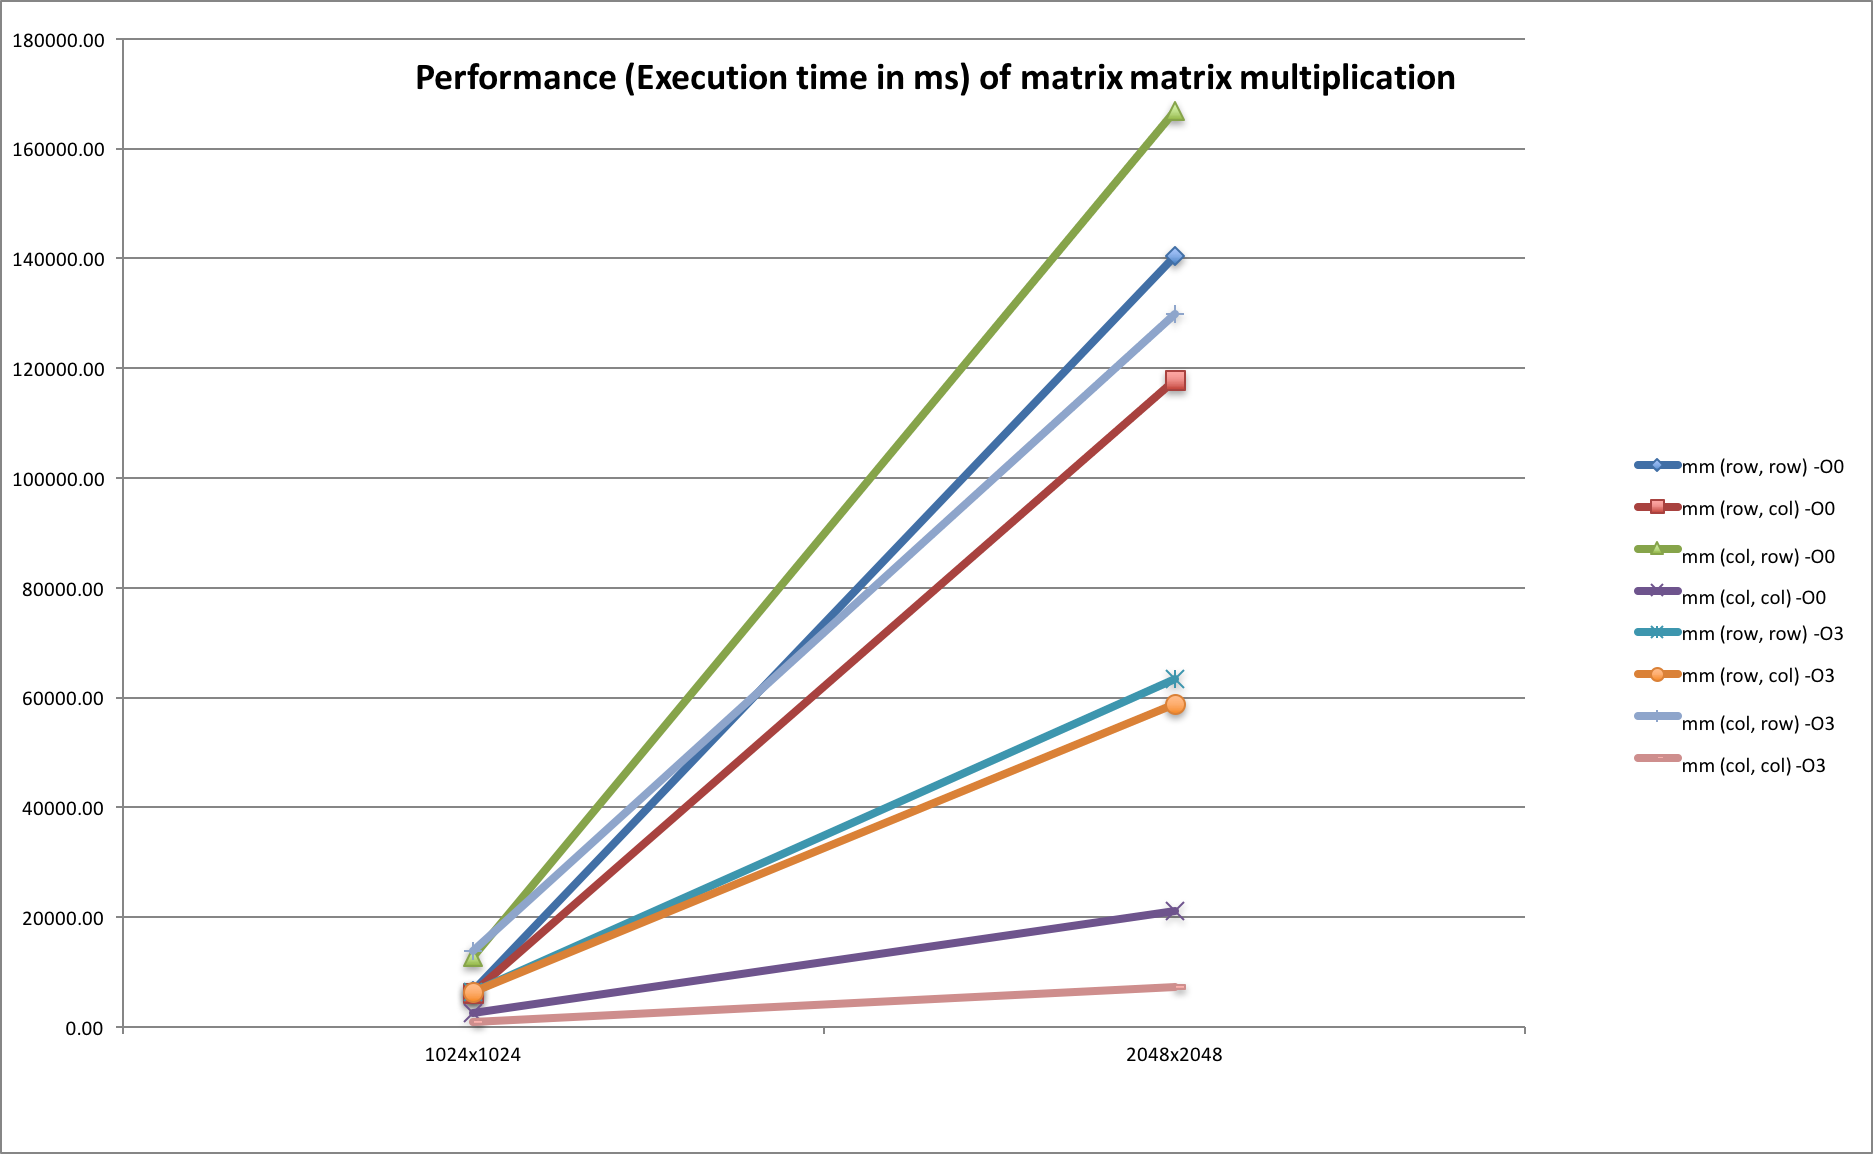
\includegraphics[scale=0.5]{mm.png} \\
\end{center}

With matrix vector multiplication the row major matrix is faster than both implementations of the optimized column major matrix. This probably comes from the fact that by doing row major element searches in both the matrix and vector are continuous instead of having to access elements out of order.
\begin{center}
    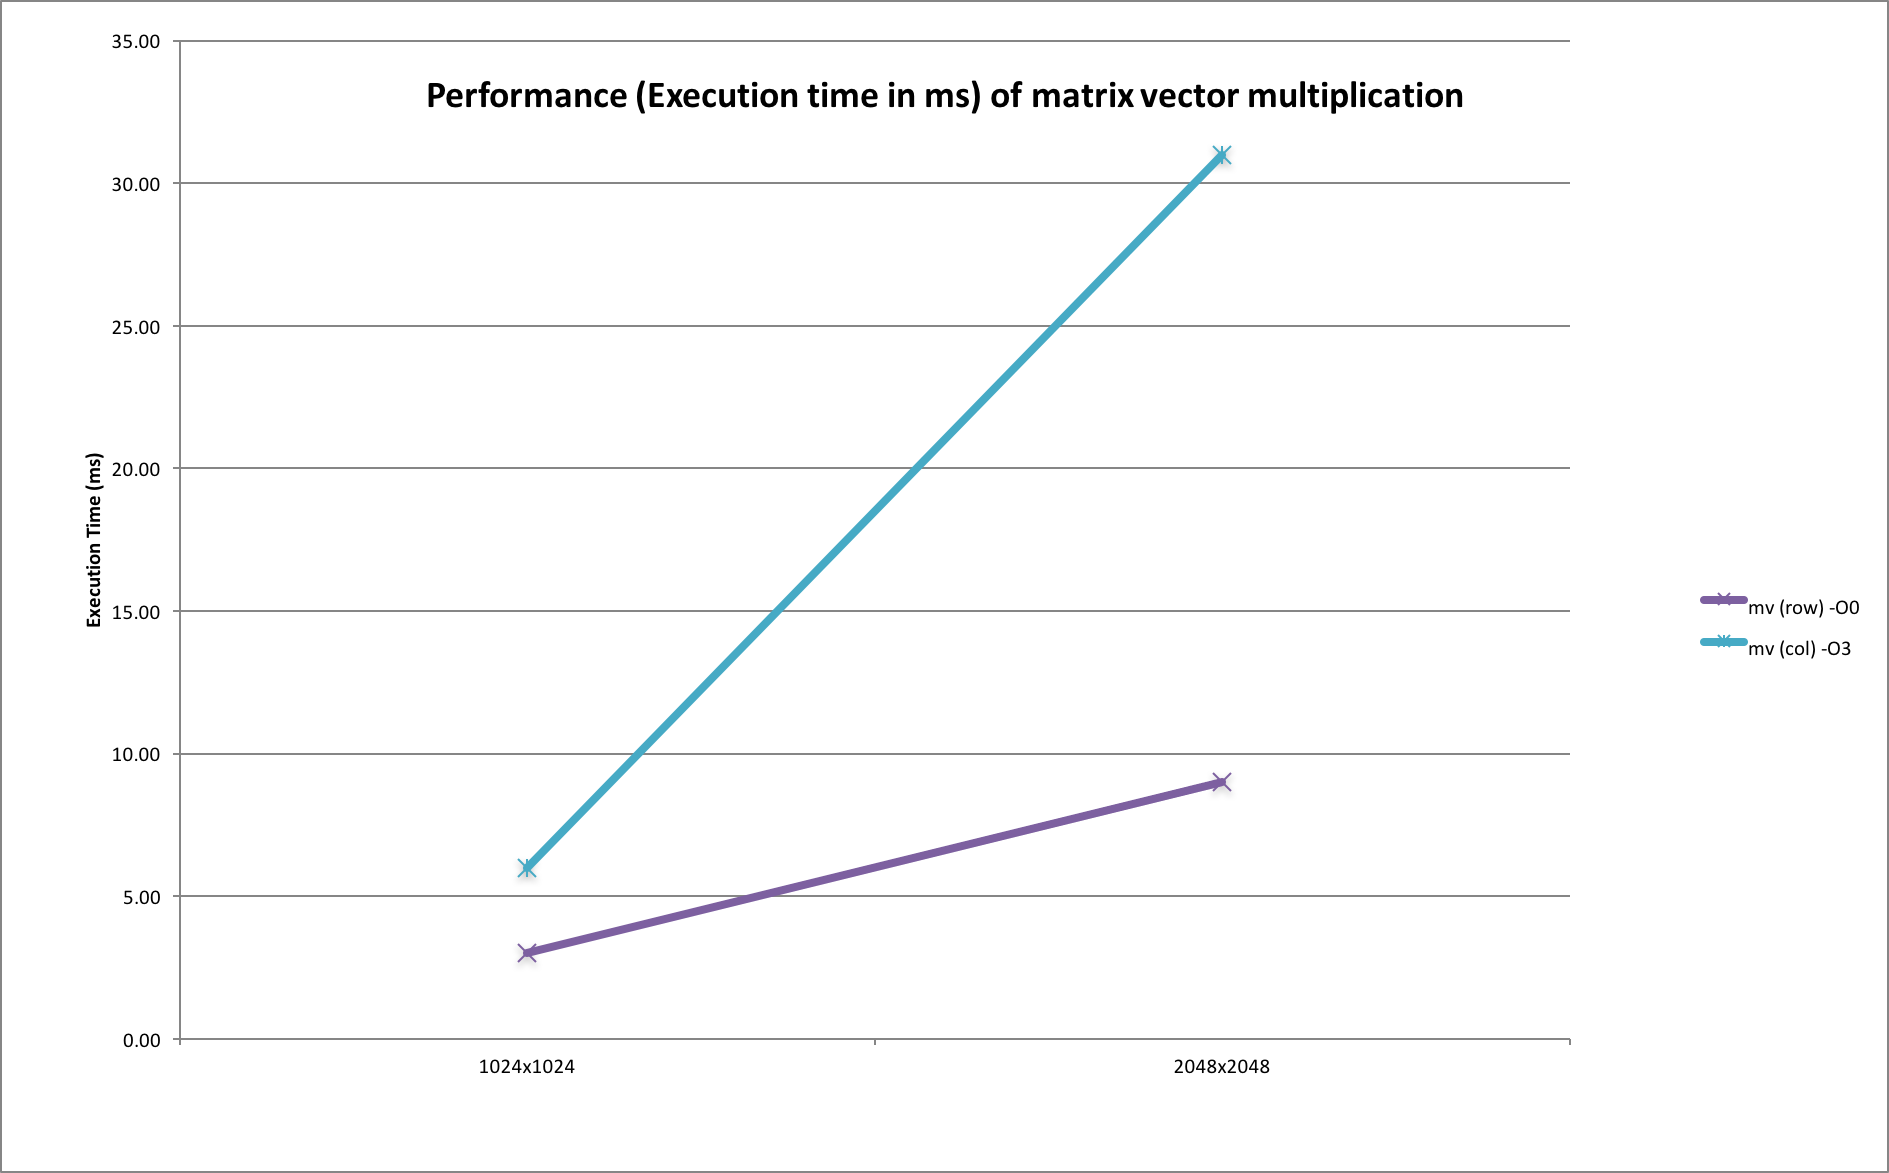
\includegraphics[scale=0.5]{mv.png} \\
\end{center}


\end{document}
              
            
